\documentclass[12pt,a4paper]{article}
\usepackage[utf8]{inputenc}
\usepackage[french]{babel}
\usepackage[T1]{fontenc}
\usepackage{amsmath}
\usepackage{amsfonts}
\usepackage{amssymb}
\usepackage{graphicx}
\usepackage[left=1cm,right=1cm,top=2cm,bottom=2cm]{geometry}
\author{KONDI Abdoul malik \\ NGANDEU NDJEUKAM Alhasan}
\title{Étude prévisionnel du projet de gestion d'une librairie}
\begin{document}
\maketitle
\tableofcontents
\newpage

\section{Planning}

\begin{center}
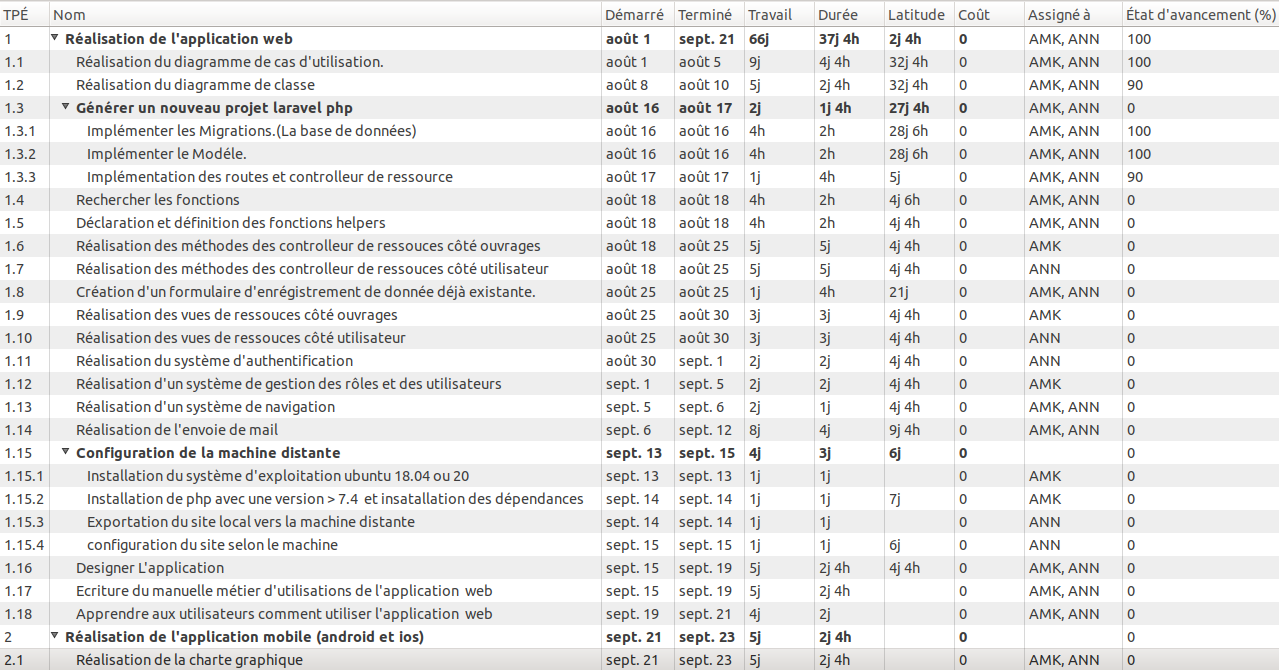
\includegraphics[scale=0.43]{images/taches.png}
\end{center}

\newpage

\section{Résumé récapitulatif du planning:}
\begin{center}
\begin{tabular}{|p{2.2cm}|p{2.2cm}|p{6.5cm}|p{6.5cm}|}
\hline 
\textbf{Début} & \textbf{Fin} & \textbf{Tâche à accomplir} & \textbf{Besoins des stagiaires} \\ 
\hline 
01/08/2022 & 13/08/2022 & Réalisation du modèle & maître de stage\\ 
\hline 
15/08/2022 & 17/08/2022 & Initialisation du projet et création de la base de données & maître de stage \\ 
\hline
18/08/2022 & 25/08/2022 & \begin{itemize}
\item[•] Ajout d'un nouvel ouvrage.
\item[•] Consulter un ouvrage.
\item[•] Rechercher un ouvrage.
\item[•] Faire l'inventaire.
\item[•] Enregistrement d'un employé(personnel).
\item[•] Enregistrement d'un nouvelle abonné.
\item[•] Attribution des droit aux utilisateur sur les fonctionnalités
\item[•] Prêter un ouvrage à un abonné.
\item[•] Restituer un prêt.
\end{itemize} & Liste des livres à la Bibliothèque \\ 
\hline 
29/08/2022 & 02/09/2022 & \begin{itemize}
\item[•] Prolonger l'emprunt d'un ouvrage.
\item[•] Renouveler l'abonnement d'un abonné.
\item[•] Alerter un abonné en cas de retard.
\item[•] Lire un ouvrage.
\item[•] Télécharger un ouvrage.
\item[•] consulter la liste des emprunt d'un abonné.
\item[•] consulter la liste des emprunts en cours.
\item[•] Pénaliser un retard.
\end{itemize} & 
\begin{itemize}
\item[•] Livres numérique
\item[•] Documents audio visuel
\end{itemize} \\
\hline 
05/09/2022 & 07/09/2022 & Utiliser la charte graphique pour l'application & - \\
\hline 
08/09/2022 & 12/09/2022 & Rédaction du manuel d'utilisation & - \\ 
\hline 
13/09/2022 & 19/09/2022 & Déploiement de l'application & 
\begin{itemize}
\item[•] Machine virtuel pour l'hébergement.
\item[•] Machine physique pour le personnel de la médiathèque.
\end{itemize} \\ 
\hline
20/09/2022 & 23/09/2022 & Formation des utilisateurs & personnels\\ 
\hline  
26/09/2022 & 30/09/2022 & Début de réalisation de l'application mobile(android \& ios) & -\\ 
\hline 
\end{tabular} 
\end{center}

\section{Conception}
\subsection{Diagramme de cas d'utilisation}
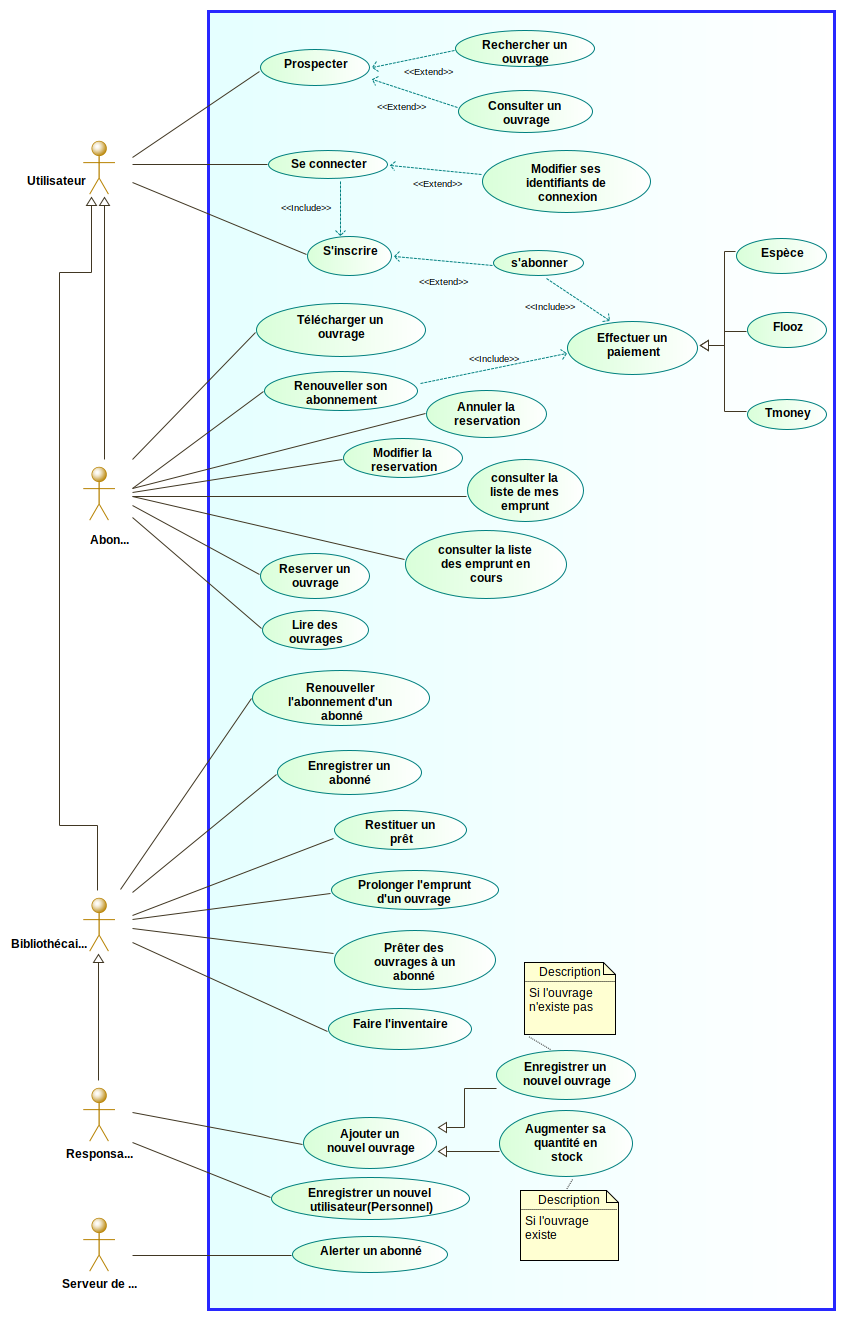
\includegraphics[scale=0.5]{../../design/UseCase.png}
\subsection{Diagramme de classe}
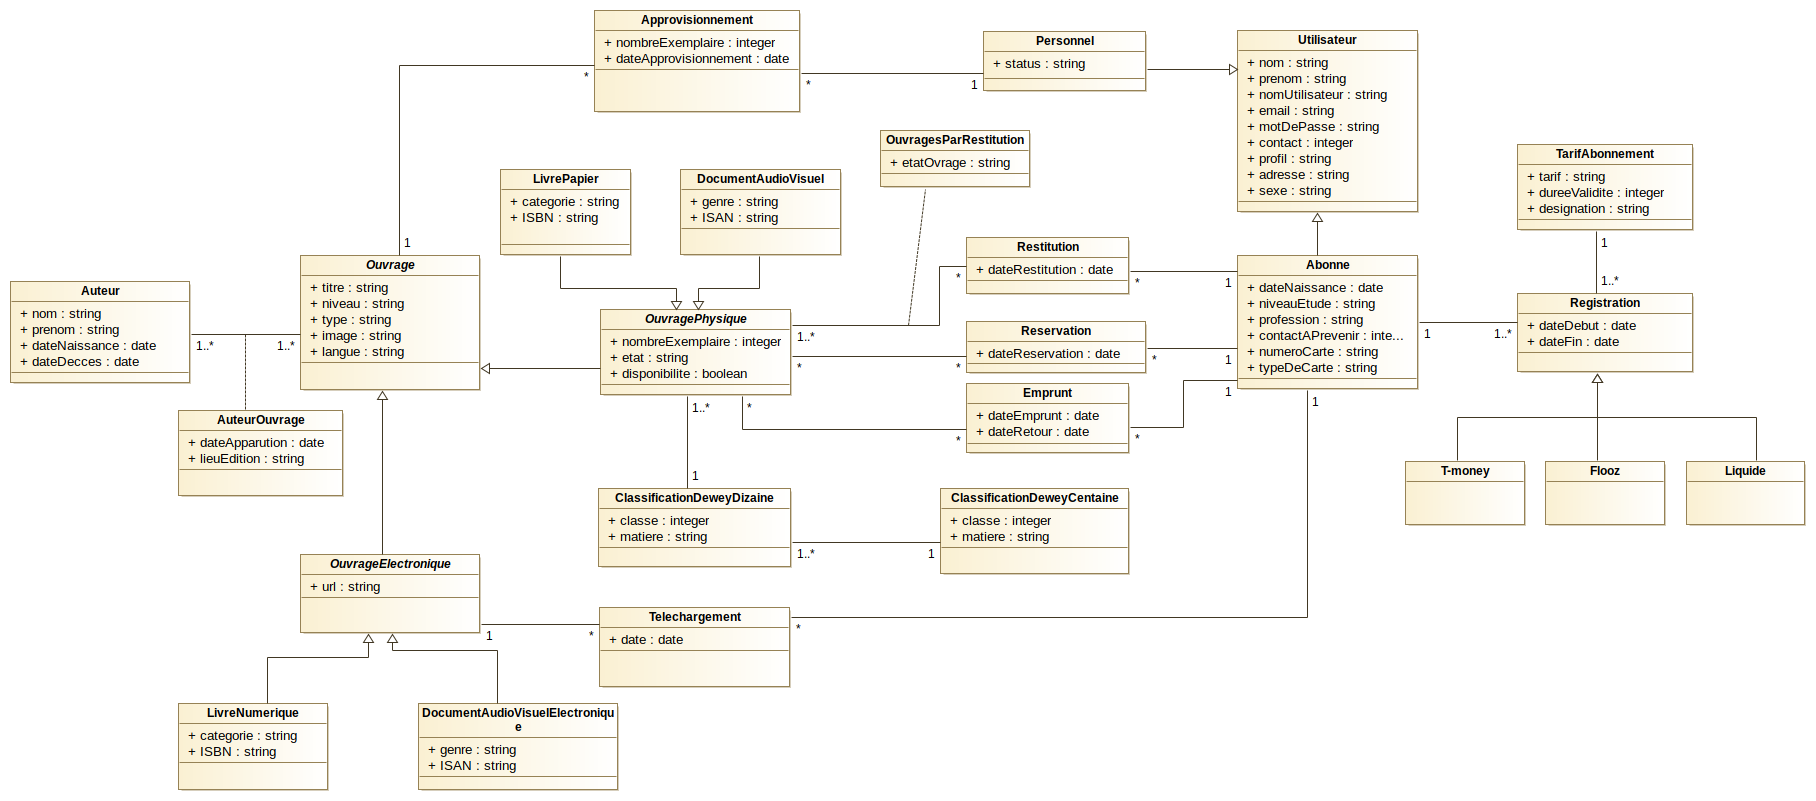
\includegraphics[scale=0.3]{../../design/ClassD.png}

\end{document}




